\documentclass{standalone}
\usepackage{tikz}

\begin{document}
\begin{minipage}{0.75\textwidth}
	\centering
	\scalebox{0.7}{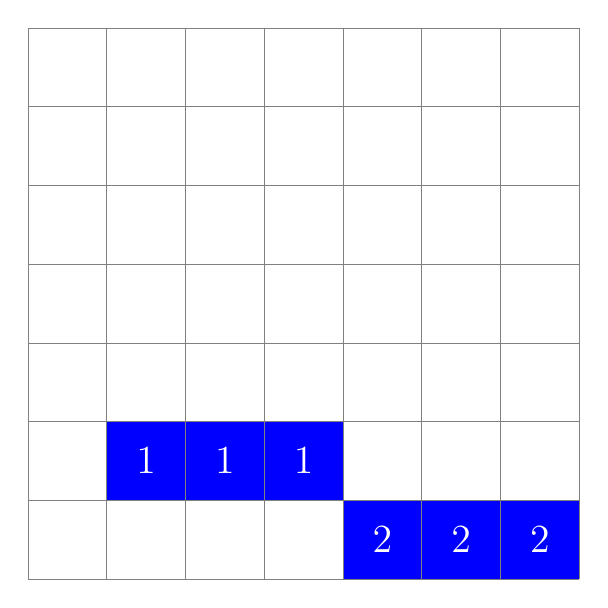
\begin{tikzpicture}	
		\foreach \x in {0,1,2}
		\fill[blue] (0+\x,1) rectangle (1+\x,2);  
		\foreach \x in {0,1,2}
		\fill[blue] (3+\x,0) rectangle (4+\x,1);
		\draw[step=1cm,gray,very thin] (-1,-0) grid (6,7);   
	
		\node[white] at (0.5,1.5) {\Large{1}}; 
		\node[white] at (1.5,1.5) {\Large{1}}; 
		\node[white] at (2.5,1.5) {\Large{1}}; 
		\node[white] at (3.5,0.5) {\Large{2}}; 
		\node[white] at (4.5,0.5) {\Large{2}}; 
		\node[white] at (5.5,0.5) {\Large{2}}; 
		\end{tikzpicture}}
	\hspace{1cm}
	\scalebox{0.7}{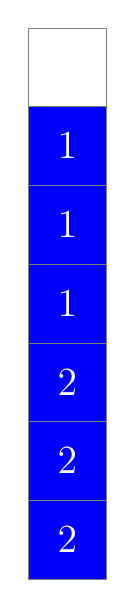
\begin{tikzpicture}
		\foreach \x in {0,1,2,3,4,5}
		\fill[blue] (8,\x) rectangle (9,\x+1);  
		\draw[step=1cm,gray,very thin] (8,-0) grid (9,7);
		\node[white] at (8.5,5.5) {\Large{1}}; 
		\node[white] at (8.5,4.5) {\Large{1}}; 
		\node[white] at (8.5,3.5) {\Large{1}}; 
		\node[white] at (8.5,2.5) {\Large{2}}; 
		\node[white] at (8.5,1.5) {\Large{2}}; 
		\node[white] at (8.5,0.5) {\Large{2}}; 
		\end{tikzpicture}}
\end{minipage}
\end{document}
